\section{Problem Statement}

In this work, we address the challenge of training an agent using
an offline Deep Reinforcement Learning (DRL) algorithm with access 
to a pre-collected dataset \( \mathcal{D} \) of experiences. 
Each experience in \( \mathcal{D} \) captures an interaction with
the environment and is represented as a tuple
\[ T = (s_t, s_{t+1}, a_t, r_{t+1}) .\] Here, \( s_t \)
and \( s_{t+1} \) are the \textbf{observed states} at time-steps
\( t \) and \( t+1 \), respectively, \( a_t \) is the \textbf{action}
taken at time \( t \), and \( r_{t+1} \) is the \textbf{reward} received
after taking action \( a_t \) and transitioning to state \( s_{t+1} \).
States can be represented in various forms:
\begin{itemize}
    \item \textbf{Numerical data}: consisting of a stack of vectors of
    real numbers representing the physical state of the environment
    (e.g., position, velocity, orientation in robotics,
    suffering from anemia or not in healthcare).
    \item \textbf{Images}: consisting of a sequence of images
    observed by the agent (e.g., frames from a camera mounted on a
    robot or a patient's medical images).
    \item \textbf{Images and numerical data}: a combination of the
    above two representations (e.g., images from a robot's camera
    and its joint angles).
\end{itemize}
The number of images (or vectors) in the state representation
is denoted by \( N_{\mathcal{S}} \) such that
\[ s_t = \{ \mathcal{S}_{t-(N_{\mathcal{S}-1})}, \ldots,
\mathcal{S}_{t-1}, \mathcal{S}_t \} \text{  and  }
s_{t+1} = \{ \mathcal{S}_{t-(N_{\mathcal{S}-2})}, \ldots,
\mathcal{S}_t, \mathcal{S}_{t+1} \} \]
\[
    \text{where } \mathcal{S}_t =
    \{\text{`num': } \mathcal{X}_t, \text{ `img': } \mathcal{I}_t\} \text{ or }
    \mathcal{S}_t = \{\text{`num': } \mathcal{X}_t\}
    \text{ or } \mathcal{S}_t = \{\text{`img': } \mathcal{I}_t\}.
\]

In real-world scenarios, where comprehensive simulators are unavailable,
the dataset \( \mathcal{D} \) may lack crucial experiences due
to potential risks (e.g., collisions, patient harm) or high costs.
This deficiency can prevent the agent's training and result in policies
that are neither effective nor robust. Therefore, our goal is to \textbf{augment}
\( \mathcal{D} \) by generating additional experiences that
\textbf{align with the environment's underlying transition dynamics}.

To model these state-transition dynamics, we use a
\textbf{Structural Causal Model} (SCM)
defined as:
\[
S_{t+1} = f_s(S_t, A_t, U_{t+1})
\]
where \( S_{t+1} \), \( S_t \), and \( A_t \) are random variables representing
the states and action, while \( U_{t+1} \) represents unobserved
variables affecting the transition.
The function \( f_s \) captures the causal mechanism
determining the next state \( S_{t+1} \) from its causes
\( S_t \), \( A_t \), and \( U_{t+1} \).
Additionally, we model the reward as:
\[
R_{t+1} = f_r(S_t, S_{t+1}, A_t)
\]
If \( f_s \) and \( f_r \) are known, we can generate
\textbf{counterfactual} experiences.

Given an observed tuple \( T = (s_t, s_{t+1}, a_t, r_{t+1}) \),
we aim to create a new tuple \( T' = (s_t, s'_{t+1}, a'_t, r'_{t+1}) \)
representing what might have occurred if a different action \( a'_t \)
were taken in state \( s_t \). This involves the following steps:
\begin{enumerate}
    \item \textbf{Abduction}: Estimate \( U_{t+1} = \hat{u}_{t+1} \)
    from the observed data \( T = (s_t, s_{t+1}, a_t, r_{t+1}) \);
    \item \textbf{Action}: Perform the counterfactual action
    \( a'_t \neq a_t \);
    \item \textbf{Prediction}: Use the estimated \( \hat{u}_{t+1} \)
    and the updated SCM model to predict \( s'_{t+1} \) and \( r'_{t+1} \).
\end{enumerate}

By creating these counterfactual samples, we can form an augmented dataset
\( \mathcal{D}' \), which can then be used to train an offline DRL agent.

In practice, however, neither the Structural Causal Model (SCM),
i.e., \( f_s \) and \( f_r \), nor the function to perform
the abduction step and estimate the unobserved variable
\( U_{t+1} \) are known. In the following, we present the framework
we devised to infer the SCM model from the available data \( \mathcal{D} \)
and simultaneously learn a function to estimate
\( U_{t+1} \) (see Subsection \ref{sec:wre}). Additionally, we investigated
a method where the noise is known and counterfactual states are collected
(see Subsection \ref{sec:e2e}).
This approach shifts the problem towards developing the most accurate and
representative simulator.

\section{Simulation Environments}

Here we introduce the simulation environments used in our experiments,
which are essential for creating the dataset \( \mathcal{D} \) and
training the offline DRL agents.

Two categories of environments are considered: \textbf{Robotics} and
\textbf{Healthcare}.

\subsection{Robotics Environments}

\textbf{MuJoCo} (Multi-Joint dynamics with Contact)
is a physics engine developed by \cite{todorov2012mujoco}
that has become a standard tool in reinforcement learning research.
It provides a platform for simulating complex multi-joint dynamics
and it's widely used in application areas which
demand fast and accurate simulation of articulated
structures interacting with their environment.

The environments we focus on in this work are
\textbf{HalfCheetah}, and \textbf{Pusher},
their wrapper can be found
in the OpenAI Gym toolkit, as initially
presented in \cite{brockman2016openaigym}.
In addition to these, we also include \textbf{Acrobot},
a classic control problem also available in the OpenAI Gym
toolkit and based on the work of \cite{sutton1998}.
Its inclusion provides
a contrast to the more complex MuJoCo environments and
allows us to test our methods on a wider range of
control problems.

\subsubsection{Acrobot}

The Acrobot environment \cite{acrobotfarama} simulates a two-link
pendulum with only the second joint actuated. A screenshot of the
Acrobot environment is shown in Figure \ref{fig:acrobot}.\\
\textbf{Description}: The Acrobot system consists of two links
connected linearly to form a chain, with one end of the chain fixed
and the other end free. The joint between the two links is actuated.
The goal is to swing the free end of the chain above the fixed base
by applying torques on the actuated joint.\\
\textbf{State space}: The state space consists of 6 continuous variables:
\begin{itemize}
    \item $\cos(\alpha_t)$, $\sin(\alpha_t)$, $\cos(\beta_t)$, $\sin(\beta_t)$
    \item Angular velocity of $\alpha_t$ and $\beta_t$
\end{itemize}
The placement of the angles can be seen in Figure \ref{fig:acrobot}.
The angles are measured counterclockwise.\\
\textbf{Action space}: The action space is discrete with 3 possible actions:
\begin{enumerate}
    \item Apply a negative torque of -1 to the actuated joint
    \item Apply no torque (0) to the actuated joint
    \item Apply a positive torque of +1 to the actuated joint
\end{enumerate}
\textbf{Reward function}: The reward function is defined as:
\begin{equation}
    R = -1 \times \text{ number of timesteps (with a limit on 100)}
\end{equation}
\textbf{Termination conditions}: The episode terminates when either
the goal position is reached or the maximum number
of timesteps (500) is reached.

\begin{figure}[h]
    \centering
    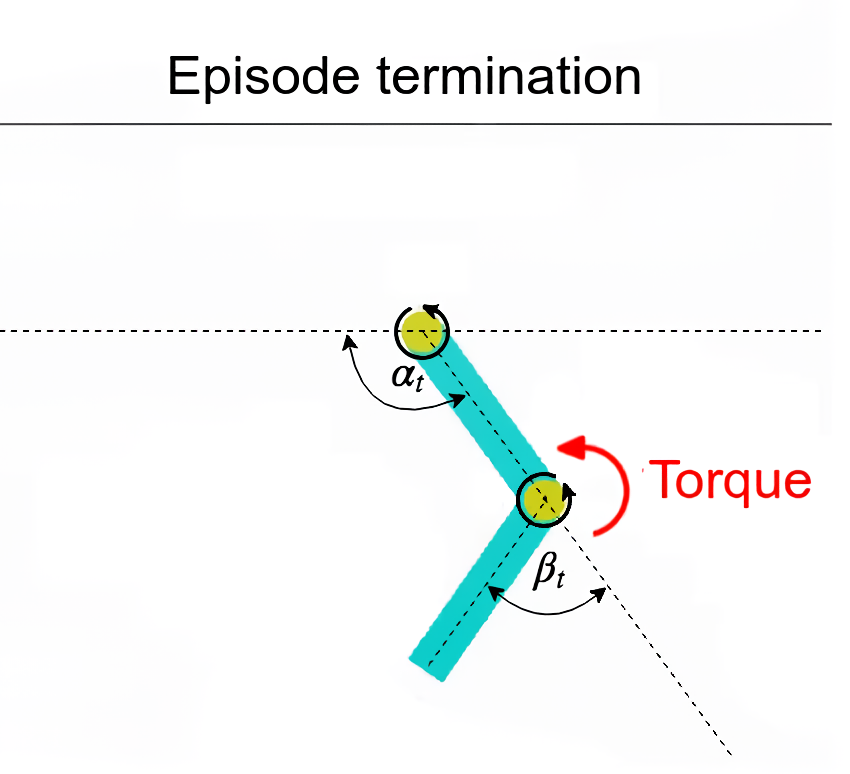
\includegraphics[width=.45\textwidth]{figures/ch4/acrobotpic.png}
    \caption{Screenshot of the Acrobot environment with information about the state.}
    \vspace{-10px}
    \caption*{\scriptsize{Source: \cite{acrobotpic}}}
    \label{fig:acrobot}
\end{figure}

\subsubsection{Half Cheetah}

The Half Cheetah environment \cite{halfcheetahfarama} 
simulates a 2-dimensional robot with two paws.
A screenshot of the Half Cheetah environment is shown
in Figure \ref{fig:halfcheetah}.\\
\textbf{Description}: The Half Cheetah is a 2-dimensional robot
composed of 9 body segments connected by 8 joints, including two paws
The objective is to apply torques to these joints to propel the
cheetah forward (to the right) as quickly as possible.
The torso and head of the cheetah remain fixed
and torque can be applied only to the other 6 joints,
which include the connections between the torso and
the front and back thighs, the thighs and shins, and the shins and feet.\\
\textbf{State space}: The state space consists of positional values
of different body parts of the Half Cheetah, followed by the velocities
of those individual parts (their derivatives), with all the positions
ordered before all the velocities.\\
\textbf{Action space}: The action space consists of $6$ continuous values
included in $[-1, 1]$,
corresponding to the torques applied to each one of the joints.\\
\textbf{Reward function}: The reward is typically
 the \textbf{forward} reward
- a reward for moving forward, minus the \textbf{ctrl} cost
- a cost for applying excessively large actions.
The reward function is defined as:
\begin{equation}
    R = \textsf{healthy\_reward} + \textsf{forward\_reward} - \textsf{ctrl\_cost}
\end{equation}
where
\begin{equation}
    \textsf{ctrl\_cost} = \textsf{ctrl\_cost\_weight} \times sum(\textsf{action}^2)
\end{equation}
and \textsf{ctrl\_cost\_weight} is a hyperparameter with a default value of $0.1$.\\
\textbf{Termination conditions}: The episode terminates if the
Half Cheetah falls over
(typically defined as when the torso's z-coordinate falls below a threshold)
or if any of the state space values is no longer finite.

\begin{figure}[h]
    \centering
    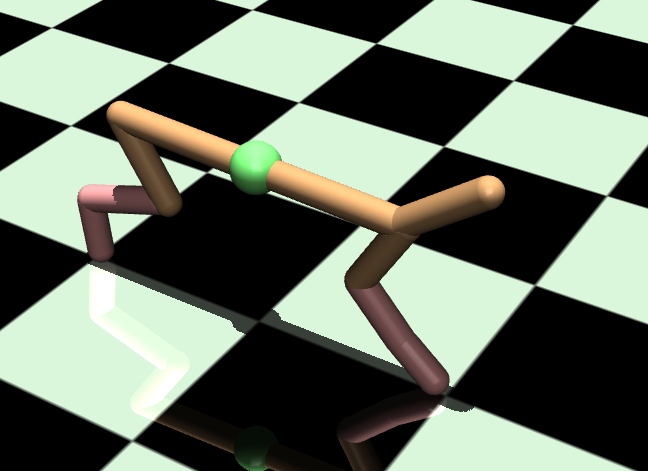
\includegraphics[width=.4\textwidth]{figures/ch4/halfcheetah.png}
    \caption{Screenshot of the Half Cheetah environment.}
    \vspace{-10px}
    \caption*{\scriptsize{Source: \cite{halfcheetahpic}}}
    \label{fig:halfcheetah}
\end{figure}

\subsubsection{Pusher}

The Pusher environment \cite{pusherfarama} simulates
a robotic arm tasked with pushing a puck to a target
location on a plane.
A screenshot of the Pusher environment is shown in Figure \ref{fig:pusher}.\\
\textbf{Description}: The Pusher consists of a
robotic arm with shoulder, elbow, forearm, and wrist joints,
and its task is to move a puck to a specified
target location on a flat surface.
The arm must apply forces to push the puck while
coordinating its own movement.\\
\textbf{State space}: The state space consists
of the angular rotation and velocities of the robotic arm's joints,
the position of the fingertips, of the puck and the position of the target.\\
\textbf{Action space}: The action space consists of $7$ continuous values,
this time given in couples $(a,b)$ - where 
$a$ and $b$ represent the torques applied at the hinge joints,
included in $[-2, 2]$.\\
\textbf{Reward function}: The reward consists of three components:
\textbf{near} reward - which measures the distance between the
pusher's fingertip and the object as a negative vector norm
($-norm(\textsf{fingertip} - \textsf{target})$),
\textbf{dist} reward - which measures the distance between
the object and the target goal calculated as a negative norm
($- norm(\textsf{object} - \textsf{target})$)
and \textbf{control} reward - which penalizes large actions
and is calculated as the negative squared Euclidean norm of the action
($- sum(\textsf{action}^2)$). The total reward is:
\begin{equation}
    R = \textsf{reward\_dist} + 0.1 \times \textsf{reward\_control} + 0.5 \times \textsf{reward\_near}
\end{equation}
\textbf{Termination conditions}: The episode terminates when the puck
reaches the target location, when 100 timesteps are reached
or when any of the state space values is no longer finite.

\begin{figure}[h]
    \centering
    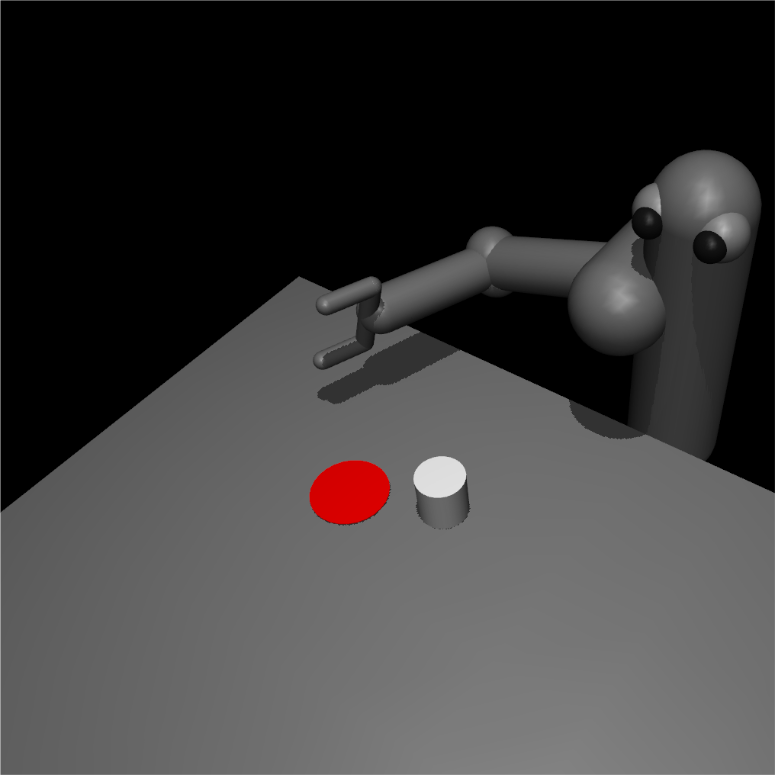
\includegraphics[width=.4\textwidth]{figures/ch4/pusher.png}
    \caption{Screenshot of the Pusher environment.}
    \vspace{-10px}
    \caption*{\scriptsize{Source: \cite{pusherpic}}}
    \label{fig:pusher}
\end{figure}

\subsection{Healthcare Environments}

The only healthcare environment we focus on in this work is
the \textbf{Diabetes} environment.

\subsubsection{Diabetes}

In our study, we employ a simulated dataset that models
the progression of type II diabetes and the effects of antiglycaemic drugs,
as seen in \cite{sim2012}.
This simulation represents a simplified version of a longitudinal
medical study with time-varying confounders.

The key features of the simulated dataset:
\begin{enumerate}
    \item Variables:
    \begin{itemize}
        \item $U_0$: Binary indicator of subject's health status
        prior to randomization (unmeasured)
        \item $A_0,\; A_1$: Binary indicators for antiglycaemic
        drug prescription at visits 0 and 1 (actions)
        \item $L_1$: Binary indicator for anaemia at visit 1 (state)
        \item $Y$: $\log HbA_{1c}$ measured at visit 2 (outcome) (final state)
    \end{itemize}

    \item Data generation process:
    \begin{itemize}
        \item $U_0 \sim \text{Bernoulli}(0.4)$
        \item $A_0 \sim \text{Bernoulli}(0.5)$ (randomized initial treatment)
        \item $L_1 | U_0, A_0 \sim \text{Bernoulli}(P(L_1 = 1) = 0.25 + 0.3A_0 - 0.2U_0 - 0.05A_0U_0)$
        \item $A_1 | A_0, L_1 \sim \text{Bernoulli}(P(A_1 = 1) = 0.4 + 0.5A_0 - 0.3L_1 - 0.4A_0L_1)$
        \item $Y | U_0, A_0, A_1 \sim \text{Normal}(\mu = 2.5 - 0.5A_0 - 0.75A_1 + 0.2A_0A_1 - U_0, \sigma = 0.2)$
    \end{itemize}
\end{enumerate}

We want to estimate the counterfactual mean of \( Y \) under
different treatment strategies \( (a_0, a_1) \).

The counterfactual means are calculated by averaging over the
distribution of \( U_0 \):
\begin{equation}
\mathbb{E}[Y(a_0, a_1)] = 2.5 - 0.4 - 0.5a_0 - 0.75a_1 + 0.2a_0a_1.
\end{equation}
Alternatively, given \( U_{0,i} \), the potential outcomes
\( Y_i(a_0, a_1) \) can be considered as being independently
generated for each \((a_0, a_1)\) and for each \(i\) from
a normal distribution with a mean of
\( 2.5 - 0.5a_0 - 0.75a_1 + 0.2a_0a_1 + U_{0,i} \)
and a standard deviation of $0.2$.

The simulation satisfies the `no unmeasured confounding' assumption,
making it suitable for evaluating causal inference methods.
This is achieved by ensuring that the data generating models for
$A_0$ and $A_1$ do not include $U_0$.
Thus, \( A_0 \) is independent of \( U_0 \) and \( A_1 \) is
independent of \( U_0 \) given \( L_1 \). Since, conditional on
\( U_0 \), the variation in \( Y(a_0, a_1) \) is independent of
all other random variables, this implies that \( A_0 \) is independent
of \( Y(a_0, a_1) \) and \( A_1 \) is independent of \( Y(a_0, a_1) \)
given \( A_0 \) and \( L_1 \).
In Figure \ref{fig:diabetes1} the SCM for the diabetes dataset
is presented.

\begin{figure}[h]
    \centering
    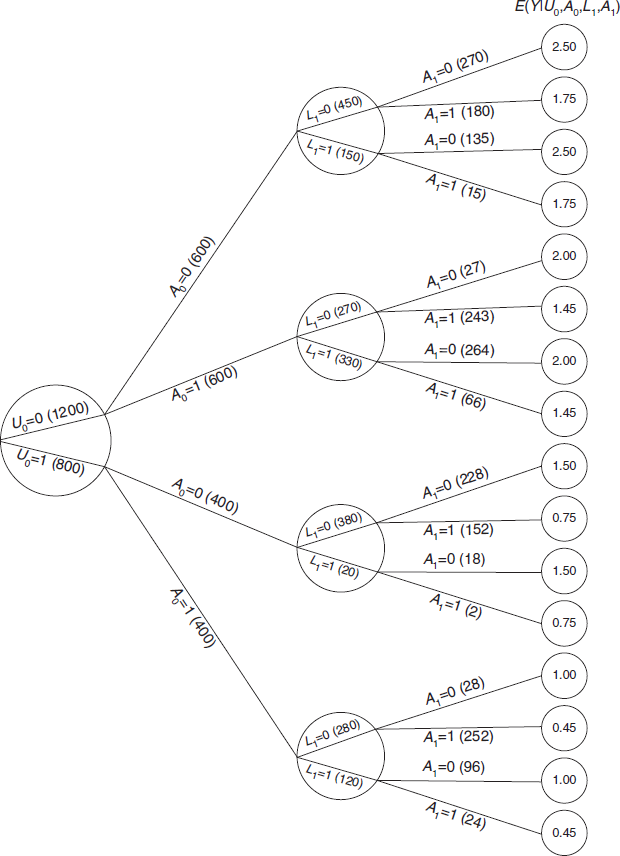
\includegraphics[width=.2\textwidth]{figures/ch4/diabetes1.png}
    \caption{Structural Causal Model for the diabetes dataset.}
    \vspace{-10px}
    \caption*{\scriptsize{Source: \cite{sim2012}}}
    \label{fig:diabetes1}
\end{figure}

This dataset captures key aspects of diabetes treatment, including:
\begin{itemize}
    \item The effect of initial health status on anaemia risk
    and $HbA_{1c}$ levels
    \item The potential side effect of antiglycaemic drugs causing anaemia
    \item The influence of anaemia on subsequent treatment decisions
    \item The causal effect of treatment on $HbA_{1c}$ levels
\end{itemize}
In Figure \ref{fig:diabetes2}, we present a tree
depicting the expected values of the variables out of
a total of $2000$ subjects.

\begin{figure}[h]
    \centering
    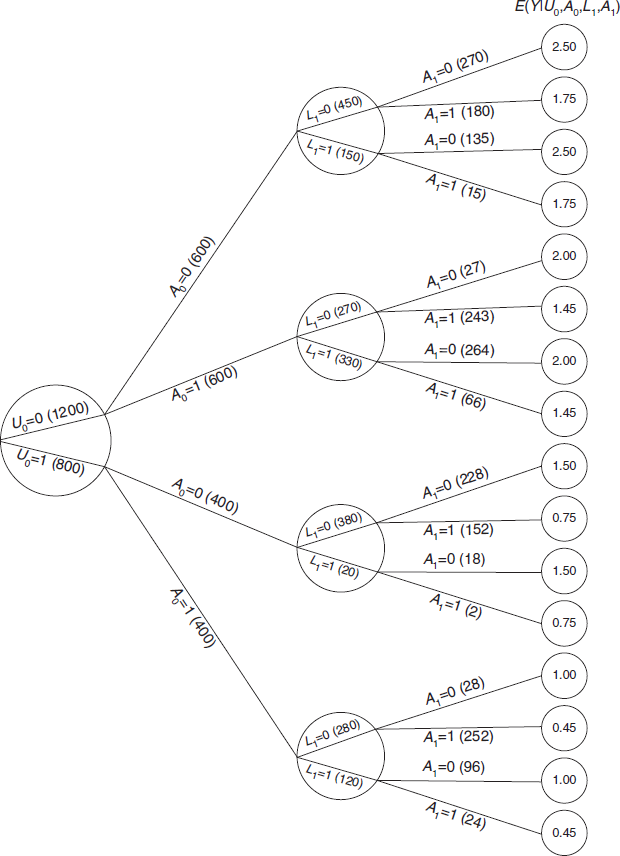
\includegraphics[width=.52\textwidth]{figures/ch4/diabetes2.png}
    \caption{Tree diagram of the expected numbers
    (out of a total of 2000 subjects) along each
    branch for the distribution from which the diabetes
    dataset was generated.}
    \vspace{-10px}
    \caption*{\scriptsize{Source: \cite{sim2012}}}
    \label{fig:diabetes2}
\end{figure}

\section{Frameworks for Counterfactual Data Generation}

In this section, we introduce two different approaches designed to
address the challenges of training agents using Offline
Deep Reinforcement Learning (DRL) with a pre-collected dataset \( \mathcal{D} \).
Both approaches aim to generate additional high-fidelity experiences
that align with the environment's underlying transition dynamics
but differ in their methodologies and assumptions.

In the following subsections, we delve into the specifics
of each approach, outlining their methodologies, advantages, and
implementation details. This exploration aims to
provide a comprehensive understanding of how these
frameworks can be employed to augment the dataset \( \mathcal{D} \) and improve
the training of offline DRL agents.

\subsection{Wasserstein Reward-enhanced CounTerfactual\\ Data Generation}
\label{sec:wre}

The first approach, called  focuses on inferring the Structural Causal Model
(SCM) from the available data \( \mathcal{D} \) and simultaneously learning
a function to estimate the unobserved variables $U_{t+1}$.

This approach is valuable when the underlying dynamics of the
environment are complex and not fully known, allowing us to
infer and utilize causal relationships for better training.

The proposed strategy for estimating the Structural Causal Model (SCM)
integrates two key components: an optional Convolutional AutoEncoder (CAE)
for dimensionality reduction and a Deep Generative Model for
implementing the causal mechanisms.

The CAE is designed to compress high-dimensional visual inputs,
making the data more manageable while retaining essential information.
The Deep Generative Model is used to learn the causal mechanism \( f_s \),
the abduction function needed to estimate \( U_{t+1} \),
and the reward model \( f_r \).
Figure \ref{fig:wre} provides a visual illustration of the entire solution.

\begin{figure}[ht]
    \centering
    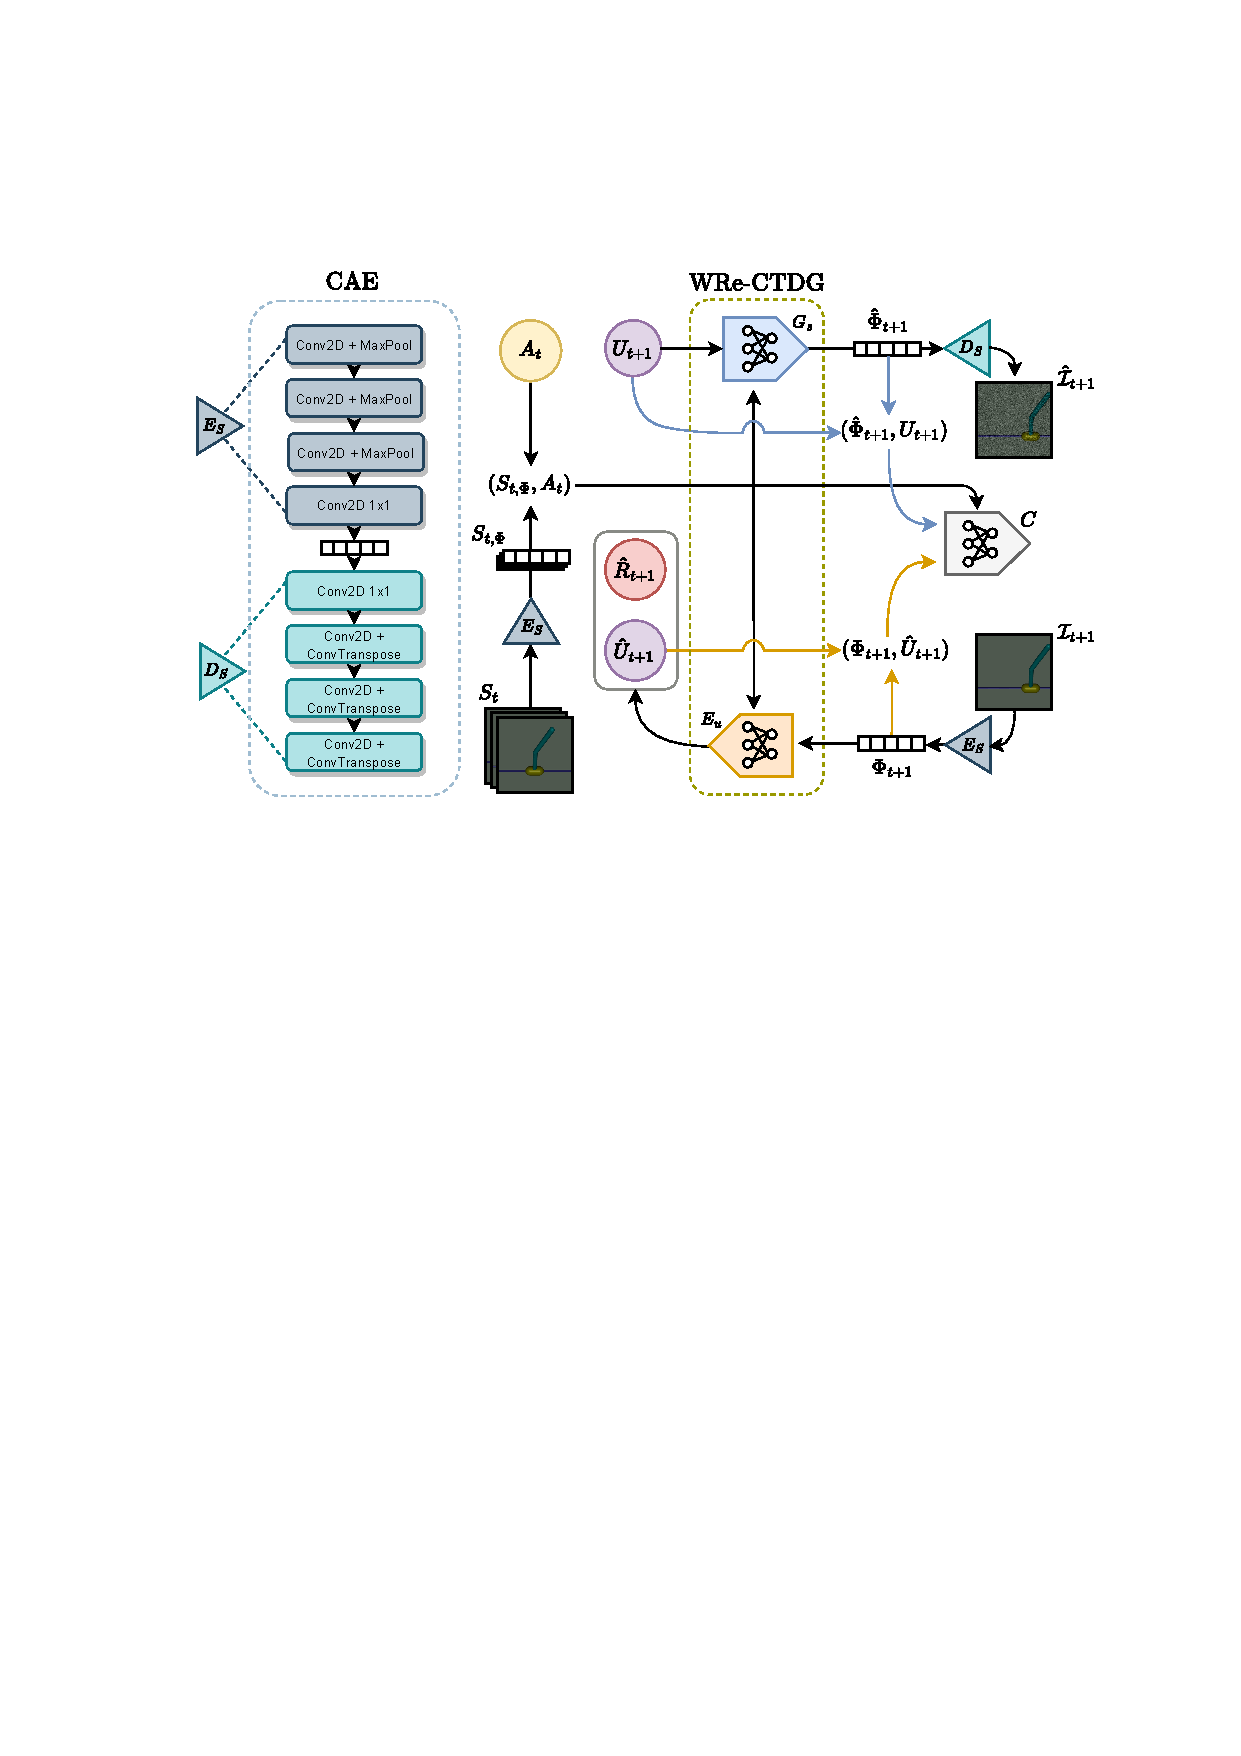
\includegraphics[width=.95\textwidth]{figures/ch4/1.wre.pdf}
    \caption{WRe-CTDG framework in a situation where the states are
    images only and the CAE is employed.}
    \label{fig:wre}
\end{figure}

\subsubsection{Dimensionality Reduction via Convolutional AutoEncoders}

Unlike state-of-the-art approaches, our work generates experience samples
where states can also be represented by images. To handle the challenges posed
by high-dimensional visual data, we present the possibility of using a CAE,
which is a Variational AutoEncoder (VAE, see Section \ref{sec:vae})
made by two Convolutional Neural Networks (CNN, see Section \ref{sec:cnn}).
to compute low-dimensional encodings that preserve the meaningful
information from the input images.
It consists of an encoder \( \phi = E_s(\mathcal{I}) \)
that extracts a low-dimensional encoding \( \phi \)
from the image \( \mathcal{I} \), and a decoder
\( D_s(\phi) = \mathcal{I}_{\text{rec}} \)
that reconstructs the original image \( \mathcal{I} \).

The CAE is trained by minimizing the reconstruction error over
the images \( \mathcal{I} \) in the collected dataset \( \mathcal{D} \):

\begin{equation}
\mathcal{L}_{E_s, D_s} = \mathbb{E}_{\mathcal{I} \sim P_{\text{data}}}
\left[ \| \mathcal{I} - \mathcal{I}_{\text{rec}} \|^2 \right]
\end{equation}

Minimizing this reconstruction error ensures that the encoder \( E_s \)
computes robust and informative image encodings, and the decoder \( D_s \)
can accurately reconstruct images from these encodings.

The encoder is used to encode the images representing the environment
states into their corresponding low-dimensional encodings.
We refer to the encoded states at time \( t \) and \( t+1 \) as
\( s_{t,\phi} = E_s(s_t) \) and \( s_{t+1,\phi} = E_s(s_{t+1}) \).
The decoder is used to reconstruct images from the low-dimensional
encodings generated by the generator network. The weights of both
\( E_s \) and \( D_s \) are frozen and not updated during the next
phase of learning the SCM model.

In the next section we are not going to explicitly use
\( s_{t,\phi} \) and \( s_{t+1,\phi} \) since utilizing the
CAE is optional and depends on the nature of the state representation.
So, by default, we will refer to the states as \( s_t \) and \( s_{t+1} \).

\subsubsection{Counterfactual Data Generation}

To learn the SCM from the collected dataset \( \mathcal{D} \),
we propose a novel strategy called
Wasserstein Reward-enhanced Counterfactual Data Generation (WRe-CTDG).
This solution builds upon the BiCoGAN framework presented in \cite{lu2020}
with significant enhancements
aimed at improving the effectiveness of the estimated SCM in generating
counterfactual samples in vision-based DRL problems. Key enhancements
include adapting the Wasserstein Generative Adversarial Network (WGAN)
framework (see Section \ref{sec:wgan})
for improved training stability and introducing an additional
loss term to learn the reward model and predict reward values for counterfactual
actions.

The WRe-CTDG framework consists of three main components:

\begin{itemize}
    \item \textbf{Generator \( G_s \)}:
    Implements the causal mechanism \( f_s \).
    It maps the inputs \( (U_{t+1}, X_t) \)
    to the next-state encoding \( \hat{\phi}_{t+1} \),
    where \( X_t = (S_t, A_t) \).
    The distribution learned by \( G_s \) is
    \( P(\hat{\Phi}_{t+1} | U_{t+1}, X_t) \).
    \item \textbf{Encoder \( E_u \)}: Implements the abduction function.
    It maps the inputs \( (\Phi_{t+1}, X_t) \) to the
    estimated unobserved factor \( \hat{u}_{t+1} \).
    The distribution learned by \( E_u \) is
    \( P(\hat{U}_{t+1} | \Phi_{t+1}, X_t) \).
    Additionally, \( E_u \) estimates the reward model \( f_r \)
    to predict the reward associated with a \( (\Phi_{t+1}, X_t) \)
    tuple, denoted as \( \hat{r}_{t+1} \).
    \item \textbf{Critic \( C \)}: Integrates the WGAN paradigm
    into the framework. It replaces the discriminator in
    traditional GANs and computes a score quantifying
    the likelihood of the input tuples being drawn
    from either the joint distribution
    \( P(\hat{\Phi}_{t+1}, U_{t+1}, X_t) \) (generated samples) or
    \( P(\Phi_{t+1}, \hat{U}_{t+1}, X_t) \) (real samples).
    
    The metric is approximated by the Wasserstein distance \( W \)
    as follows:
    \begin{equation}
        \begin{aligned}
            W &=& \mathbb{E}_{T \sim P_{\mathcal{D}}} \left[ C(\hat{\Phi}_{t+1}, U_{t+1}, X_t) \right] \\ 
            & &- \mathbb{E}_{T \sim P_{\mathcal{D}}} \left[ C(\Phi_{t+1}, \hat{U}_{t+1}, X_t) \right]
        \end{aligned}
    \end{equation}
    where $C(\cdot)$ is a score computed by the critic.
\end{itemize}

The goal of training the encoder-generator pair is to minimize \( W \),
thereby improving the ability of both the encoder and generator
to produce samples that are indistinguishable from those generated
by their counterparts. Additionally, the function \( E_u \) must
accurately predict the rewards for each transition.
Thus, the objective function for the pair \( (G_s, E_u) \) is defined as:

\begin{equation}
L_{G_s, E_u} = -W + \lambda_R \; \mathbb{E}_{R_{t+1} \sim P_{\mathcal{D}}}
\left[ \| \hat{R}_{t+1} - R_{t+1} \|^2 \right]
\end{equation}

where \( \lambda_R \) regulates the influence of the reward
prediction term. On the other hand, the critic is trained
using the Wasserstein Loss with Gradient Penalty,
which addresses the problem of vanishing gradients and
the limited expressive power of traditional WGANs \cite{gulrajani2017}.
The objective function for \( C \) is defined as:

\begin{equation}
L_C = W + \lambda_G \mathbb{E}_{T \sim P_{\mathcal{D}}}
\left[ (\| \nabla_{\tilde{\Phi}_T, \tilde{U}_T} C(\tilde{\Phi}_T,
\tilde{U}_T, X_t) \| - 1)^2 \right]
\end{equation}

where \( \lambda_G \) determines the strength of the Gradient Penalty
and the interpolation variables \( \tilde{\Phi}_T \) and \( \tilde{U}_T \)
are given by:

\[
    \begin{aligned}
        \tilde{\Phi}_T \;\; &=& \alpha \, \Phi_{t+1} + (1 - \alpha) \, \hat{\Phi}_{t+1} \\ 
        \tilde{U}_T \;\; &=& \alpha \, U_{t+1} + (1 - \alpha) \, \hat{U}_T
    \end{aligned}
\]

for \( \alpha \in [0, 1] \), sampled uniformly at random,
indicating a blend between real and generated samples.
By maximizing \( W \), the critic aims to increase the difference
in evaluations between samples generated from the generator distribution
\( P(\hat{\Phi}_{t+1} | U_{t+1}, X_t) \) and those from the encoder
distribution \( P(\hat{U}_{t+1} | \Phi_{t+1}, X_t) \).

When the data is purely numerical or when the
CAE is employed, both the Generator $G_s$ and the
Encoder $E_u$ consist exclusively of fully connected
layers. This architecture is sufficient to handle
the numerical input and effectively capture the dependencies
in the data. However, when the state representation
includes images, convolutional layers are incorporated
into both the Generator and the Encoder:
\begin{itemize}
    \item In the Encoder, the convolutional blocks perform a
    downsampling on the images, effectively reducing their
    spatial dimensions while capturing essential features.
    These downsampled feature maps are then flattened
    and combined with the other numerical data,
    ensuring a comprehensive representation of the input.

    \item In the Generator, after extracting the numerical data,
    convolutional blocks are used to upsample the output of
    the fully connected network. This upsampling process
    reconstructs the spatial dimensions,
    enabling the model to generate the image $\mathcal{I}_{t+1}$.
\end{itemize}

\subsubsection{Experience Generation through Counterfactual Augmentation}

After understanding the causal mechanism \( f_s \),
the abduction function, and the reward model \( f_r \),
we can utilize WRe-CTDG and (optionally) the CAE
for counterfactual
data augmentation. The original dataset \( \mathcal{D} \)
is expanded by a factor of \( \beta \)
according to the method described in Algorithm \ref{alg1}.
Specifically, if the CAE is used, for each sampled tuple
\( T = (s_t, s_{t+1}, a_t, r_{t+1}) \in D \),
the image encodings in $s_t$, so
\( s_t[\text{`img'}] = \{I_{t-(N_{\mathcal{S}}-1)}, \ldots, I_{t-1}, I_t\} \),
and \( I_{t+1} \in s_{t+1} \) are first computed using
the encoder \( E_s \). Next, \( E_u \) and \( G_s \)
are used to create a counterfactual
sample through three steps:
\begin{enumerate}
    \item Perform abduction with \( E_u \) to estimate
    the unknown factor \( \hat{u}_{t+1} \);
    \item Use \( G_s \) to generate the counterfactual
    states \( \hat{s}'_{t+1} \) given
    \( \hat{u}_{t+1}, s_t \), and the counterfactual
    action \( a'_t \);
    \item Use \( E_u \) again to produce the reward
    \( \hat{r}'_{t+1} \).
\end{enumerate}

Finally, if the CAE is used,
the image \( \hat{I}'_{t+1} \) is generated using
the decoder \( D_s \). Once the augmented dataset
\( \mathcal{D}' \)
is ready, it can be used to train any off-policy DRL
algorithm, such as D3QN or TD3.

\begin{algorithm}[hb]
    \small
    \caption{WRe-CTDG + CAE Counterfactual Augmentation} \label{alg1}
    
    \vspace{1pt}
    \KwIn{dataset $\mathcal{D}$, augmentation factor $\beta > 1$, \\
    ($E_s$, $D_s$) CAE, ($G_s$, $E_u$) WRe-CTDG}
    \KwOut{augmented dataset $\mathcal{D}'$}
    
    
    \BlankLine
    $\mathcal{D'} \gets copy(\mathcal{D})$ \\
    $M \gets$ size of $\mathcal{D}$ \\
    $M' = M \gets$ size of $\mathcal{D'}$ \\
    \While{$M' < \beta M$}{
        Sample batch $B$ $\in \mathcal{D}$ \\
            $B' \gets \emptyset$ 
            
            \ForEach{$ T = (s_t, s_{t+1}, a_t, r_{t+1}) \in B$}{
                \If{CAE is used}{
                    $s_{t} \gets \text{encode images in $s_{t}$:} \, E_s(s_t)$ \\
                    $s_{t+1} \gets \text{encode last image in $s_{t+1}$:} \, E_s(s_{t+1})$
                }
                \textit{Abduction}: $\hat{u}_{t+1} \gets E_u(s_{t+1}, s_{t}, a_t)$ \\
                \textit{Action}: $a'_t \gets \text{choose random action} \neq a_t $ \\
                \textit{Prediction}: $\hat{s}'_{t+1} \gets G_s(\hat{u}_{t+1}, s_{t}, a'_t)$ \\
                $\hat{r}'_{t+1} \gets E_u(\hat{s}'_{t+1}, s_{t}, a'_t)$ \\
                \If{CAE is used}{
                    $\hat{s}'_{t+1} \gets \text{decode last generated image in }\hat{s}'_{t+1} \text{ : } \, D_s(\hat{s}'_{t+1})$ \\ 
                }
                Insert $T' = (s_t, \hat{s}'_{t+1}, a'_t, \hat{r}_{t+1})$ in $B'$ \\
            }
    
        Insert $B'$ in $\mathcal{D}'$ \\
        $M' \gets$ size of $\mathcal{D}'$
    }
    
    \BlankLine
    \Return $\mathcal{D}'$
    \vspace{2pt}
\end{algorithm}

\subsection{End-to-End CounTerfactual Data Generation}
\label{sec:e2e}

The second approach assumes that the noise in the system is known
in the training phase and focuses on directly collecting
counterfactual states.

This approach shifts the problem towards creating the most
accurate and representative simulator, enhancing the
realism and diversity of the generated experiences.
It is particularly useful when there is access to detailed
knowledge about the noise in the system,
even in just a subset of the available data, enabling a more
precise simulation of the environment.

\begin{figure}[ht]
    \centering
    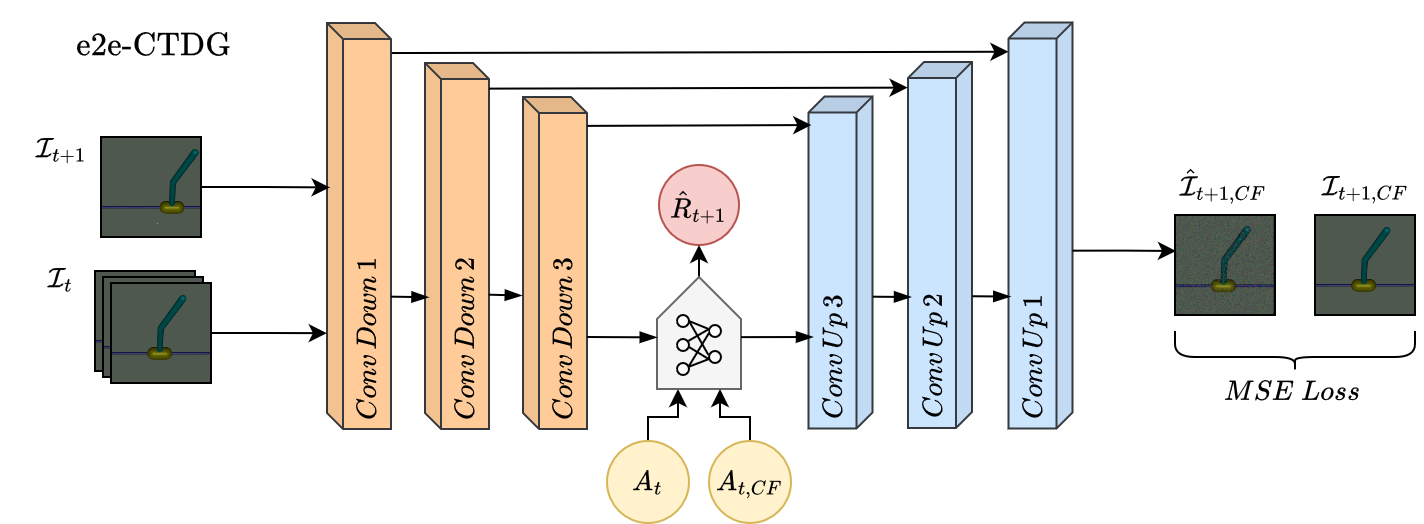
\includegraphics[width=\textwidth]{figures/ch4/2.e2e.png}
    \caption{e2e-CTDG framework in a situation where the states are
    images only.}
    \label{fig:e2e}
\end{figure}

\subsubsection{Counterfactual Data Generation}

The proposed strategy involves the employment of a Neural Network
architecture, using two additional Convolutional Neural Networks
for the tasks of downsampling and upsampling images,
the upsampling layers are connected to the downsampling layers
using the skip connection mechanism to improve the quality of the
upsampled images.

The inner neural network is designed to take as input the last state at
time $t$ ($\mathcal{S}_{t}$), the last state at time $t+1$
($\mathcal{S}_{t+1}$), the action $a$ at time $t$,
and a counterfactual action $A_t \neq A_{t,\, CF}$.
In the case of states composed by images only,
the input of the neural network is $\mathcal{I}_{t}$ and $\mathcal{I}_{t+1}$
downsampled and flattened for usage in the fully connected layers.
In the case of states composed by numerical data only,
the input of the neural network is $\mathcal{X}_{t}$ and $\mathcal{X}_{t+1}$
and the CNN layers are not used.
Finally, if the states are composed by a combination of images
and numerical data,
the input of the neural network is $\mathcal{X}_{t}$, $\mathcal{X}_{t+1}$ and
the downsampled and flattened images $\mathcal{I}_{t}$ and $\mathcal{I}_{t+1}$.

The output of the neural network is the counterfactual state
$\hat{\mathcal{S}}_{t+1,\, CF}$ and the counterfactual reward
$\hat{R}_{t+1,\, CF}$.
If the states contain images, the output of the neural network
is passed to the upsampling CNN layers to generate the counterfactual
image $\hat{\mathcal{I}}_{t+1,\, CF}$.

The loss function used to train the neural network is composed of
two terms: the Mean Squared Error (MSE) between the predicted
counterfactual state and the real counterfactual state and the
MSE between the predicted counterfactual reward and the real
counterfactual reward:
\begin{equation}
    \mathcal{L} = \mathbb{E} \left[ \left( \hat{\mathcal{S}}_{t+1,\, CF} - \mathcal{S}_{t+1,\, CF} \right)^2 \right] +
    \mathbb{E} \left[ \left( \hat{R}_{t+1,\, CF} - R_{t+1,\, CF} \right)^2 \right]
\end{equation}

The e2e-CTDG model takes as input the current state $s_t$,
the next state $s_{t+1}$, the original action $a_t$,
and the counterfactual action $a_t'$. It then produces a counterfactual
next state $\hat{s}_{t+1}'$ and a counterfactual reward $\hat{r}_{t+1}'$.
This process effectively allows the algorithm to ask ``What if?''
questions about the environment, simulating alternative scenarios
that didn't actually occur but could have occurred if different actions
had been taken. 

\subsubsection{Experience Generation through Counterfactual Augmentation}

After understanding the end-to-end causal mechanism of the e2e-CTDG model,
we can utilize it for counterfactual data augmentation.
The original dataset $\mathcal{D}$ is expanded by a factor of $\beta$
according to the method described in Algorithm \ref{alg2}.
For each sampled tuple
$T = (s_t, s_{t+1}, a_t) \in \mathcal{D}$,
the process is simplified compared to the WRe-CTDG method.
Instead of separate encoding and generation steps,
the e2e-CTDG model $G_{e2e}$ directly generates the counterfactual
state $\hat{s}_{t+1}'$ and reward $\hat{r}_{t+1}'$
given the current state $s_t$, next state $s_{t+1}$,
current action $a_t$, and a randomly chosen counterfactual action $a'_t$.
The abduction step here is implicit in the generation process.
This end-to-end approach eliminates the need for explicit
separate estimation of unknown factors.
Once the augmented dataset $\mathcal{D}'$ is ready, it can be used to
train any off-policy DRL algorithm, such as D3QN or TD3.

\begin{algorithm}[hb]
    \small
    \caption{e2e-CTDG Counterfactual Augmentation} \label{alg2}
    
    \vspace{1pt}
    \KwIn{dataset $\mathcal{D}$, augmentation factor $\beta > 1$, $G_{e2e}$
    e2e-CTDG}
    \KwOut{augmented dataset $\mathcal{D}'$}
    
    
    \BlankLine
    $\mathcal{D'} \gets copy(\mathcal{D})$ \\
    $M \gets$ size of $\mathcal{D}$ \\
    $M' = M \gets$ size of $\mathcal{D'}$ \\
    \While{$M' < \beta M$}{
        Sample batch $B$ $\in \mathcal{D}$ \\
            $B' \gets \emptyset$ 
            
            \ForEach{$ T = (s_t, s_{t+1}, a_t) \in B$}{
                \textit{Action}: $a'_t \gets \text{choose random action} \neq a_t $ \\
                \textit{Prediction}: $(\hat{s}'_{t+1}, \hat{r}'_{t+1}) \gets G_{e2e} (s_t, s_{t+1}, a_t, a'_{t})$ \\
                Insert $T' = (s_t, \hat{s}'_{t+1}, a'_t, \hat{r}_{t+1}')$ in $B'$ \\
            }
    
        Insert $B'$ in $\mathcal{D}'$ \\
        $M' \gets$ size of $\mathcal{D}'$
    }
    
    \BlankLine
    \Return $\mathcal{D}'$
    \vspace{2pt}
\end{algorithm}